\documentclass{article}
\usepackage[utf8]{inputenc}
\usepackage[utf8]{inputenc}
\usepackage{array}% 
\usepackage{tabularx}
\usepackage[dvipsnames]{xcolor}
\usepackage{afterpage}
\usepackage{booktabs}
\usepackage{minted}
\usepackage{palatino} %prety font without ligatures: easier copy-paste from PDF to other formats
\usepackage{graphicx} % import images for figures
\usepackage{setspace} % line spacing
  \renewcommand{\baselinestretch}{1.0} % single-spaced lines
\usepackage{hyperref} % make URLs and citations clickable
\usepackage[sort&compress]{natbib}% 
\usepackage[utf8]{inputenc}
\usepackage{fancyhdr} % page headers
\usepackage{multirow}
\pagestyle{fancy} % Activate page headers of the "fancy" type
\fancyhead{} % header: empty


%\title{The Putative \textit{Drosophila} Larva Central Complex}
\title{The central complex of the larval fruit fly brain}

\author{Laura Lungu;  Albert Cardona}
\date{}
\begin{document}
\maketitle


\section*{Abstract}
     The Central Complex (CX) is a conserved set of arthropod brain neuropils that integrates multisensory information and mediates spatial navigation and sleep. In holometabolous insects such as the fruit fly \textit{Drosophila}, the CX forms during metamorphosis and serves the adult stage. Whether a form of the CX exists in the brain of the evolutionarily novel larval stages is not known. Here, we analysed the connectome of the \textit{Drosophila} larval brain and, on the basis of neuronal lineages, synaptic connectivity patterns, anatomy, and neuronal-behaviour maps, we identified a simplified larval CX, comprising 4 key neuropils: the protocerebral bridge(PB), the elipsoid body(EB), the fan-shaped body(FB) and the noduli (NO). Consistent with our interpretation, we found in the larval brain synaptic connectivity patterns characteristic of the adult, including (i) strong, direct connections from MBONs to the FB and NO; (ii) strong visual input into the PB and EB; and (iii) strong connectivity between FB and NO. Interestingly, we find that some neuronal lineages contributing to the larval CX do not contribute to the adult CX, whilst many others remain conserved. The characterisation of a larval CX brings structure to larval brain circuits, linking with a vast body of literature, and will inform the design of experiments to probe brain function.
    
    
\section{Introduction}

% Introduction:
The Central Complex(CX) is a morphologically conserved set of neuropils found across insects
%(bumblebee, the red flour beetle and the Monarch butterfly) 
that acts as navigational centre and sensory integration area for coordinated motor activity.
This region is best described %(connectivity wise) 
and understood %(function wise) 
in \textit{Drosophila} adult where its core functions include multisensory navigational decisions, path integration, allocentric orientation of the head relative to its body - convergence of head and body direction - and providing an internal sense of direction in the absence of stimuli. %also promotes sleep

At the larval stage, this animal exhibits  similar behaviours to those observed in the adult: it demonstrates chemotaxis during foraging and performs aversive phototaxis in response to blue light. In addition to individual stimulus response, \textit{Drosophila} larva is able to integrate competing stimuli into a coherent representation(Gepner et al.,2015) prior to decision making. The larval brain shares similar set of neuroblasts with the adult, and presents neuropils with direct correspondance to the adult such as the Antennal Lobe(AL), the Mushroom Body(MB), and the Lateral Accessory Lobe(LAL). 

The underlying connectivity of AL, MB, LAL is well understood at present(Winding et al., 2023), as well as the Lateral Horn(LH; a larvae specific neuropil). Nevertheless, these structures constitute only up to 25\% of the larval brain connectome. We postulate that amongst the remaining ~75\% of neurons, a multitude should be devoted to navigational decisions, and may constitute the putative larval Central Complex neuropils. These are unlikely to be reocgnizable morphologically at this stage of development, since the brain lobes aren't yet fused at the midline, and the larval brain presents a commisure. The basis of our search has to be, in turn, based on lineage membership, relative spatial location and circuit architecure specific to adult central complex neuropils. We use all three in an iterative process to progressively find putative CX neurons.


The adult \textit{\textit{Drosophila}} central complex has five neuropils: the Protocerebral Bridge (PB), the Fan-shaped Body (FB; or central body upper), the Ellipsoid body(EB; or central body lower), the Noduli (NO) ~\citep{hanesch1989neuronal} and, as of recently, the Assymetrical Body (AB) ~\citep{wolff2018neuroarchitecture}. The Lateral Accessory Lobe (LAL) reciprocally interconnects with these, making it an important accesory structure and reference point. 

The central complex has been associated with a set of functions - spatial navigation decisions, directed locomotion and sleep %REF
- some of which are shared by the larva. The neuroblasts that give rise to the neuronal lineages populating the adult CX also exist in the larval brain. A subset of embryonic-born neurons from these neuroblasts remain undifferentiated throughout larval stages and delineate the structures of the adult CX, acting as pioneer neurons during metamorphosis 
~\citep{andrade2019developmentally}; however, earlier-born, differentiated neurons of the same lineages contribute to structures in the larval brain. The question remains as to what structures. Furthermore, the larval brain presents readily recognizable neuropils of accepted homology with the adult brain, including the antennal lobe ~\citep{berck2016wiring}, mushroom body ~\citep{eichler2017complete}, and lateral accessory lobe ~\citep{hartenstein2015lineage}.
 In the adult brain, the central complex neuropils are primarily medial structures, suggesting that any putative larval counterpart will be necessarily split across the midline given the lack of fusion of the larval brain hemispheres. With all the above in mind, and considering the evolution of the larval stage in holometabolous insects ~\citep{truman1999origins}as well as the presence of a central complex-like structure in the larva of the holometabolous beetle Tribolium castaneum, we set out to identify the putative central complex neuropils of the fruit fly larva on the basis of: neurons contributing to the larval neuropils that share lineage of origin with the adult CX neurons;the synaptic connectivity present across the putative larval CX neuropils; the spatial position and overall morphology of the arbors of larval CX neuropils, which is similar to that of the adult CX neurons. 


\section{Methods}
 \subsection{Nomenclature}
 We used an adapted version of the nomenclature system proposed by Wolff et al. 2015, a convention that provides a description of individual cell types. As such, in a neuron's name, the first neuropil is the neuropil closest to the cell body; the second component of a cell’s name is the predominant morphology of its arbors, abbreviated as either "d" for dendrites, or "b" for boutons(axon terminals). 
 
 Ovals in the schematics represent the cell bodies, solid and hatched fills denote spine and bouton arbor morphologies, respectively.
 %%ADD FIGURE

In the adult, thse neurons are categorised as instrinsic neurons (those that have their axon and dendrites conained within any CX neuropils), local neurons (cells that have their axon and dendrites contained within one CX neuropil), input neurons (cells that have dendritess contained within a CX neuropil but their axon the CX) and output neurons (neurons that have boutons contained within a CX neuropil but dendrites outside the CX).

Collectively, we refer to intrinsic and local neurons as 'Central Complex Core neurons'. 
 %PB: protocerebral bridge; EB: ellipsoid body; FB:fan-shaped body; NO: noduli; d:dendrites; b: boutons. 
 
 % CX core neurons - should we add to nomenclature?
 
 \subsection{Connectivity}
   We've identified stereotypical Central Complex connectivity patterns in the adult brain; this included cross-interactions between individual neuropils of the central complex, their connections with various accessory structures such as the Lateral Accessory Lobe, as well as other established anatomical structures that exist in both the adult and larval stage of this animal (Musrhoom Body, Lateral Horn,Antennal Lobe, Olfactory Lobe). Importantly, we were also interested in input patterns towards specialised neuropils such as visual input processing  of polarized light into the Protocerebral bridge and the Ellipsoid Body Ring neurons ~\citep{hardcastle2021visual, lin2013comprehensive, hulse2021connectome}, thus explored the sensory inputs from different modalities towards the distinct neuropils, intteratively checking for Central Complex Lineage derived neurons(see methods below). 
   Last but not least, we identified the output of the CX neuropils %EXAMPLES
   into various structures of the larval brain, and their respective motor outputs.(see %FIGURE)     

 \subsection{Lineage}
 The Drosophila central brain consists of stereotyped neuronal and glial lineages, originating from stem cells - neuroblasts - that appear in the early embryo. Embryonic neuroblasts express specific combinations of regulatory genes, which provide each lineage with the information needed to shape the connectivity of its neurons. %next parahgraph needs rephrasing
 Thus, lineages become structural modules: neurons of the same lineage project together in one or two fiber tracts, and form synapses in spatially restricted brain compartments. The ring neurons of the EB, for example, are derived from one lineage DALv2 (aka EBa1) and the columnar neurons of the CX are produced by four pairs of lineages located in the dorso-medial brain, called DM1, DM2, DM3 and DM4 (also reffered to as DPMm1 DPMpm1, DPMpm2 and CM4, respectively). The spatial pattern of these lineages is reflected in the position at which their corresponding tracts enter and terminate within the CX. In this manner, the four lineages subdivide the CX neuropils into four evenly sized quadrants ~\citep{andrade2019developmentally}. Using the identified lineages contributing to the CX of the Adult Drosophila ~\citep{andrade2019developmentally}(see results, and there are more sources), we filtered the neurons satisfying imposed connectivity rules (of the neurons identified to satisfy a connectivity rule, how many come from a known CX lineage) and continued to constrain these iteratively via a back and forth manual analysis of these neurons. 
 %developmental-structural units of macrocircuitry formed by the sibling neurons of single progenitors called neuroblasts.
 
 
\subsection{Searching for Dopaminergic Neurons in the Putative Central Complex}
We stained the Dopaminergic Neurons (DANs) of mostly unknown identity within the larval brain to check for their presence within the putative larval Central Complex. To do this, we adapted and optimised a protocol from Nern et al. 2015 ~\citep{nern2015optimized}, for multicolor stochastic labeling useful for the visualization of individual cell shapes and cell arrangements in Drosophila. In this method, expression of multiple membrane-targeted and distinct epitope-tagged proteins is controlled both by a transcriptional driver and by stochastic, recombinase-mediated excision of transcription-terminating cassettee. This approach is know as MultiColor FlpOut (MCFO). Fly lines with both MCFO reporters and recombinase drivers support MCFO analyses of GAL4 expression patterns in a single fly cross. Heat-shock induced expression of FLP recombinase was used to excise FRT-flanked interruption cassettes from UAS reporter constructs carrying HA, V5, and Flag epitope tags, and stained with epitope-tag specific antibodies. This labelled a subset of the cells in the expression pattern with a stochastic combination of the three labels.
We combined this original protocol with the MCFO Immunolabelling protocol for larval Drosophila from HHMI Janelia, to include that background staining and use landmarks to be able to accurately identify the position of individual neurons within the CNS. 

\subsection{Molecular Biology and Drosophila Genetics}

The following strains from the Rubin GAL4:
TH-Gal4;tsh-Gal80 expressing DANs exclusively in the brain, except for the PAM cluster. 

The following effector stocks were used: Miscellaneous-07 A-08  R57C10-FlpL

Crossing and preparation of larvae
20-30 MCFO virgin females were crossed with 10-15 TH-GAL4-tshGAL80 males and incubated at 25 degrees for 2-3 days on molases plates. The crosses were then synchronised by switching the molases plates and leaving them to incubate at 25 degrees for 3-4 hours, after which the flies are remoeved the the molases plates are kept and incubated at 25 degrees for 24 hours. After the synchronised crosses have incubated they have heathocked for 30 minutes at 37 degrees. 

After the heatshock, the plates were incubated at 25 degrees for 2 days until larvae reached early 2nd instar.

Dissection and Staining 
The CNS of several 2nd instar larvae were dissected and placed on 1x PBS. The samples were then fixed for 1 hour in 4\% Paraformyldehate, washed with 10\%PBST (4 x 15 minute washes) and blocked in 5\% Normal Bovine Serum (check brand) for 2 hours.


The following primary antibodies were used: Rabbit anti-HA(1:300); Rat anti-FLAG (1:200); Mouse α-Neuroglian (1:50) 
The following secondary antibodies were used:AF488 Donkey α-Mouse(1:500); AF594 Donkey α-Rat(1:700); DL549 Goat α-Rabbit(1:800)
The following conjugated antibody was used: AF647 Mouse α-V5 Tag(1:200)


Primary Antibodies were added and the samples were incubated on a nutator first for 4 hours at room themperature then for 1-2 overnights at 4 degrees. Samples were then washed (4x15 minutes) with 10\%PBST and the same process was repeated for Secondary Antibodies. After incubation with secondary antobodies the samples were washed again with 1\%PBST and blocked for a second time with Normal Bovine Serum for 2 hours, after which the conjugated antibodies were added using the same method described above. 

Mounting and Dehydration 
Poly-­‐L-­‐lysine (PLL) coverglass was prepared 
The larval tissue was mounted on  poly-­‐L-­‐lysine (PLL) coated cover glass. 



\section{Results}
\begin{table}
\centering
    \begin{tabular}{|c|c|cc|cc|cc|cc|}
     \hline
              Larval lineages & Adult lineages & \multicolumn{2}{c|}{PB}& \multicolumn{2}{c|}{FB}&\multicolumn{2}{c|}{EB}&\multicolumn{2}{c|}{NO}\\
     \hline
                  & & .b &  .d & .b &  .d & .b &  .d & .b &  .d \\
         Bamv12-ven & LALv1 &    &     &    &     &  2 &   2 &    &     \\
            Dalv23 & EBa1 &    &     &    &     & 12 &     &    &     \\
           Dalcl12 & - &    &     &    &     &  2 &     &    &     \\
            BAla12 & - &    &     &    &     &  2 &     &    &     \\
               CPb & -  &    &     &    &     &  8 &   4 &    &     \\
            BAlpant & -  &    &     &    &     &  2 &     &    &     \\
            CM13lat & DM6/CM3 &    &     &    &     &  4 &     &    &     \\
            CM13med & DM6/CM3 &    &     &    &     &  2 &   2 &    &     \\
              DPMm1 & DM1&    &   4 & 14 &     &    &     &  4 &     \\
             DPMpm1 & DM2&   &     &    &     &    &   4 &    &     \\
              DPLc5 & - &    &     &    &     &    &     &  2 &     \\
                CPa & - &   &     &  2 &     &    &     &    &     \\
              dall1 & - &   &     &  4 &     &    &     &    &     \\
             BAla34 & - &   &     &  4 &     &    &     &    &     \\
            bamd2-d & - &   &     &  2 &     &    &     &    &     \\
            %possibly crea1, which is bamd1
            bamd2-v & - &   &     &  2 &     &    &     &    &     \\
           dplal1-3 & - &   &     &    &     &  2 &     &    &     \\
            DPMpl12 & SIPp1 &   &     &  2 &     &    &     &    &     \\
             DPMpm2 & DM3 &   &     &    &     &    &   2 &  2 &     \\
        dplcpostmed & - &   &     &    &     &    &     &  4 &     \\
         DPMl34post & - &   &     &    &     &    &     &  2 &     \\
          bamv12dor & LALv1 &   &     &    &     &    &     &  2 &     \\
             DPMl12 & - &  2 &     &    &     &    &     &  2 &     \\
              Dalv1 & - &  8 &     &    &     &    &     &    &     \\
              %VLPA2 is the name for adult but this lineage doesn't contribute to the adult cx
            BLAd-OL & - &  2 &     &    &     &    &     &    &     \\
          BLAV12ant & - &    &     &    &   2 &    &     &    &     \\
              BLVp2 & - &   &   2 &    &     &    &     &    &     \\
              DPMm2 & - &   &   2 &    &     &    &   2 &    &     \\
            DPMl-ant & - &    &   2 &    &     &    &     &    &   2 \\
          DALcm12-v & CREa2  &    &   2 &    &   2 &    &     &    &  10 \\
               BLAl & - &    &     &    &   2 &    &     &    &     \\
                CPe & -  &    &     &    &   2 &    &     &    &   4 \\
         BAmv12-dor & - &    &     &    &   2 &    &     &    &   6 \\
           CM4-vm & DM4 &    &     &    &   2 &    &     &    &   4 \\
        Dalcm12-m & &    &     &    &     &    &   4 &    &   4 \\
            BAmd1 & CREa1&    &   2 &    &     &    &     &    &     \\
            BLP12 & -  &    &     &    &     &    &   2 &    &     \\
           dpmpl3 & - &    &     &    &     &    &     &    &   2 \\
        \bottomrule
    \end{tabular}
    \caption{Central complex lineages corresponding to each neuropil. The second column lists the corresponding lineage in the adult brain, as per Eckstein et al. 2020, listing only the subset of adult lineages known to contribute to the adult CX (note that we don't list further adult lineages that contribute to the CX whose larval corresponding lineage doesn't). The numbers are of neurons belonging to each lineage (rows) that contribute either axons (".b" for "bouton") or dendrites (".d") to the CX neuropils (columns). }
        \label{lineages}
    \end{table} 

    \begin{table}

    \begin{tabular}{l|ccccc}
        \toprule
        Neuropil & PB & FB & EB & NO & LAL \\
        \midrule
        PB &  & * & * &  & * \\
        FB & * & & & * & * \\
        EB & * & & & & \\
        NO & & * & * & & \\
        LAL & & & & & \\ % Does the LAL connect to any of PB, FB, etc. ?
        MBONs & & * & & & \\
        \bottomrule
    \end{tabular}
    
    \caption{Synaptic connectivity between CX neuropils, with a row neuropil synapting onto a column neuropil.}
    \label{inputsoutputs}
    \end{table}
    
    \begin{table}
    \centering
        \begin{tabular}{ lccr } 
         \toprule
         Neuropil &  Sensory Inputs Adult & Sensory Inputs Larva   \\ 
        \midrule
            PB & visual & visual\\
               & olfactory & olfactory \\
        \hline
            FB & olfactory & olfactory \\ 
               & thermosensory        & \\  % larva has thermosensory?
        \hline
            EB &  visual  & visual  \\
               &  olfactory  & olfactory  \\
               &  mechanosensory  &   \\
        \hline
            NO &  proprioceptive  & proprioceptive  \\
              &  olfactory  &  olfactory \\

        \bottomrule
    \end{tabular}
    \caption{Sensory inputs into the Central Complex neuropils in adult vs larva}
    \label{sensoryinputs}
    \end{table}


    \begin{figure}
        \centering
        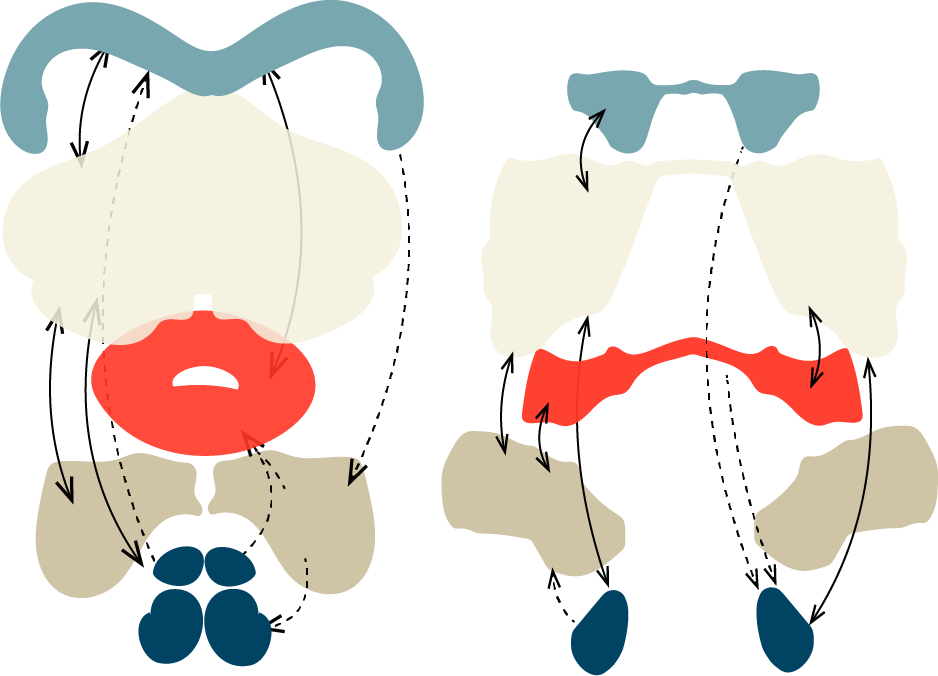
\includegraphics[width=12cm]{Images/CX_new.png}
        \caption{\textbf{The Central Complex Neuropils and their inter-connectivity}. Dotted-line arrows represent unidirectional connections, filled-line arrows indicate bidirectional connections  \textbf{A.} The adult \textit{\textit{Drosophila}} CX. Bidirectional connectivity is seen between PB-FB, PB-EB, FB-LAL and FB-NO, with unidirectional connections from NO-PB, PB-LAL, LAL-NO and NO-EB; \textbf{B.} The larval \textit{Drosophila} CX. Bidirectional connections are  PB-FB, FB-EB, FB-LAL, FB-NO and EB-LAL; unidirectional connections are seen from NO-LAL, PB-NO and EB-NO}
        \label{fig:cxdiagram}
     \end{figure}

     \begin{figure}
      \centering
      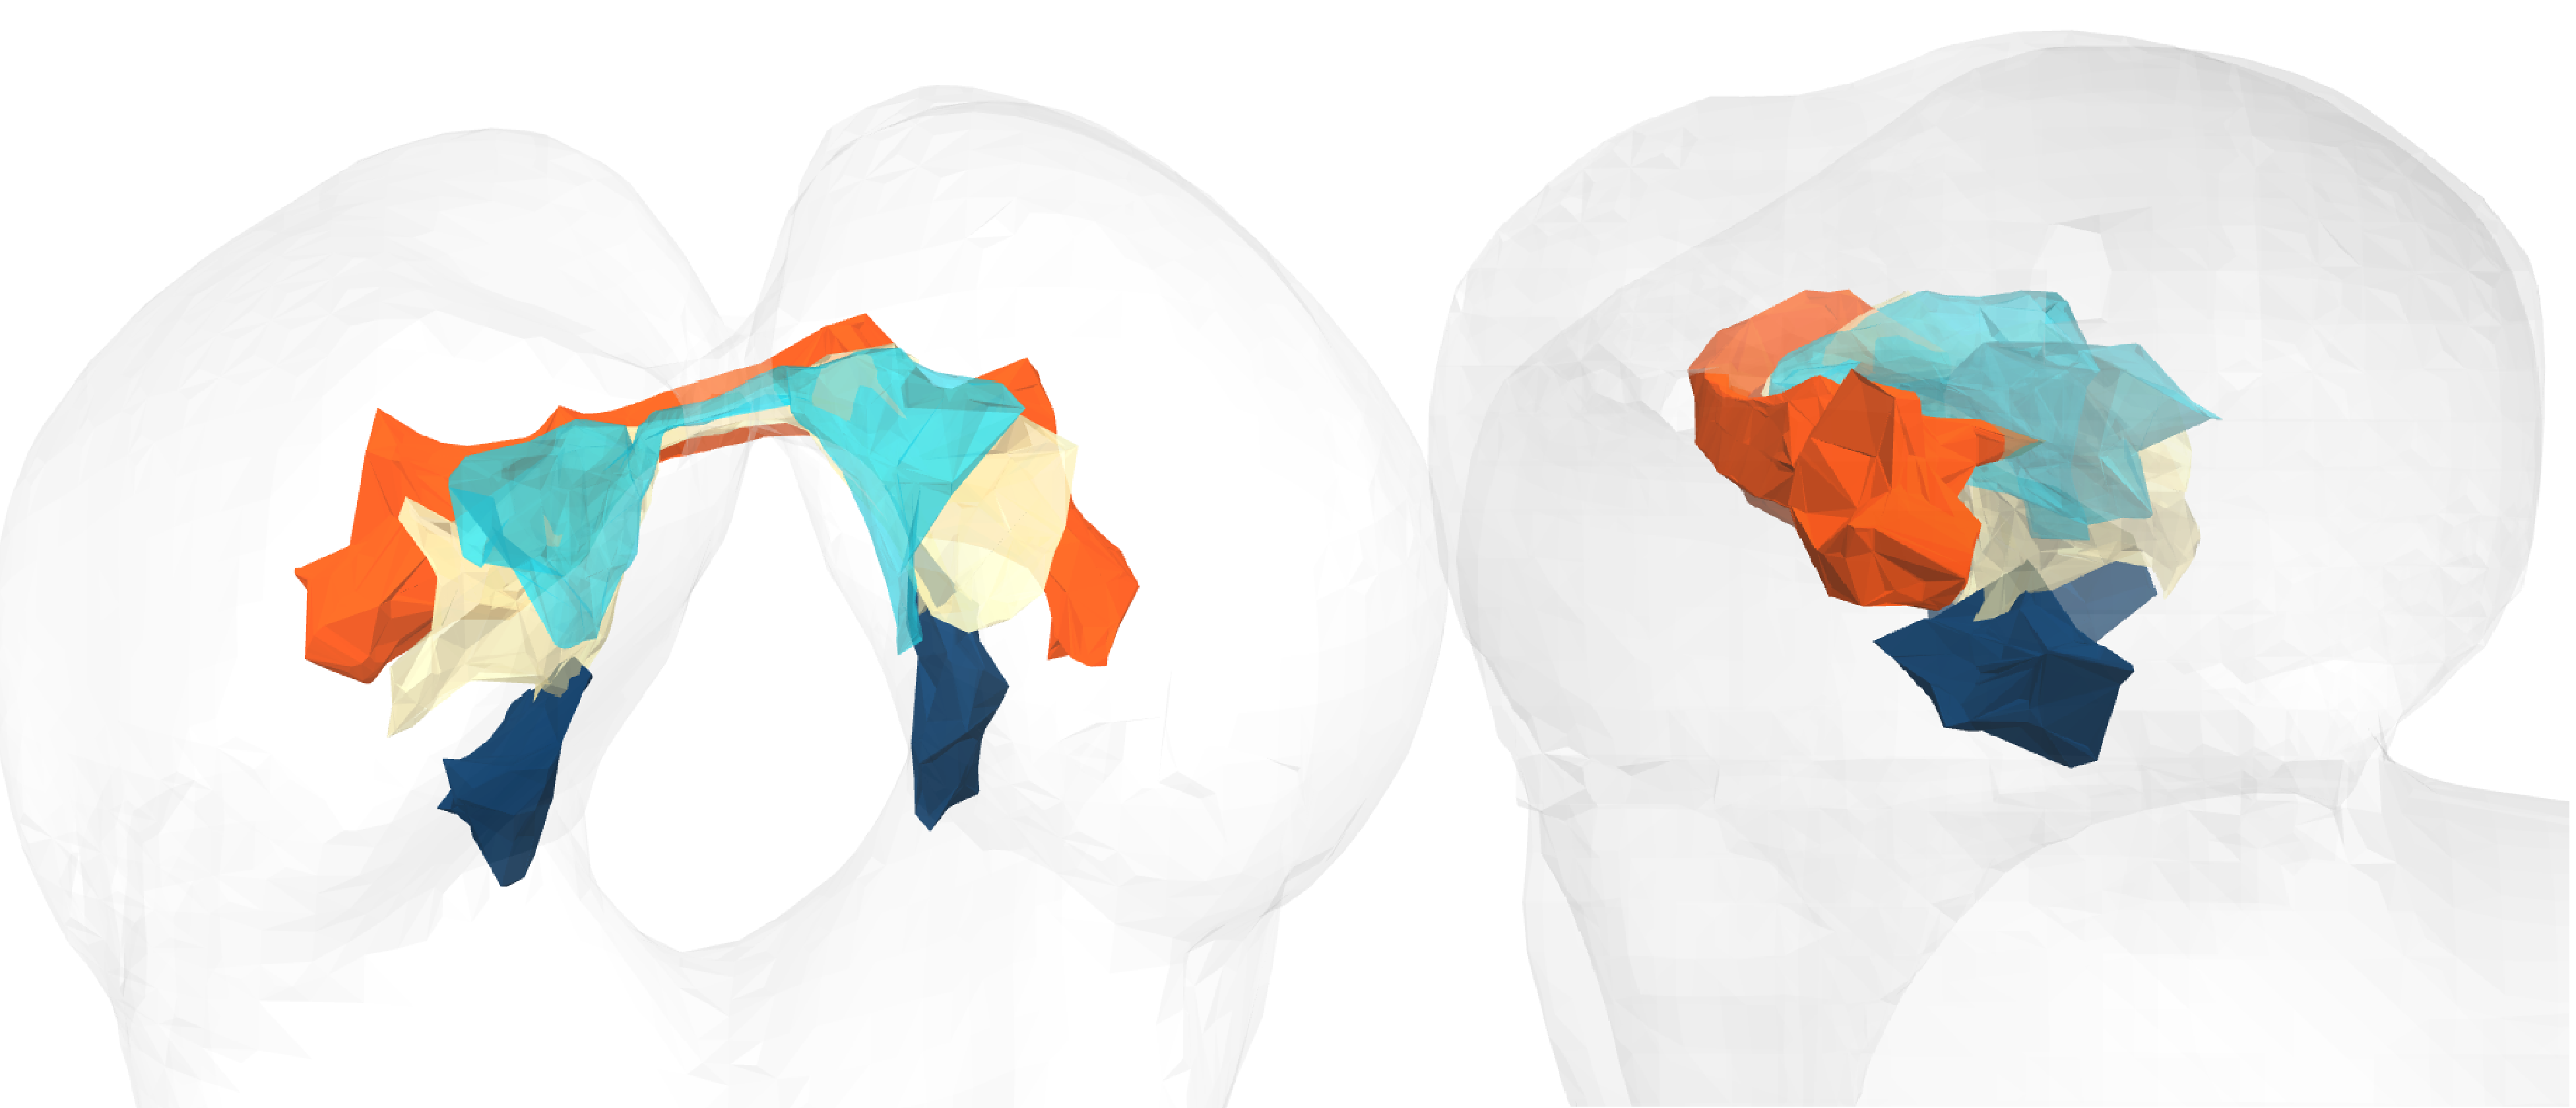
\includegraphics[width=12cm]{Images/Figure neurons/cx_orthographic.pdf}
      \caption{\textbf{The Central Complex Neuropils}. Posterior and Lateral views of the Larval Central Complex neuropils. }

     \end{figure}





    \begin{figure}
        \centering
        \includegraphics[width=12cm]{Images/Figure neurons/CentralComplexNeurons.pdf}
        \caption{\textbf{Larval CX neuron boutons define the volumes of the 4 main CX neuropils.} Posterior and lateral views of neurons that contribute boutons (".b") to each of the 4 neuropils. In concordance with the adult, the PB is the most dorsal and posterior neuropil of the whole brain; the FB occupies an intermediate medial position; the EB is the most medial anterior neuropil (same dorso-ventral level as the mushroom body medial lobe but even more anterior); and the NO are medial and ventral.}
        \label{fig:cxneurons}
     \end{figure}   


%TODO:TABLE column add 1 column with .ds and 1 column .d.bs (so basically neurons tat have both .ds and.bs in the CX cus they are core neurons)
%I need clarification - how to do this best? %i probably can figure it out  

% Lineage correspondences
\subsection{Correspondence between larval and adult neuronal lineages}

On the basis of neurons from lineages known to contribute to the adult central complex and the spatial arrangement of their arbors in the brain, we will now examine each larval central complex neuropil individually.


\subsection{The larval Protocerebral Bridge (PB)}


In the adult \textit{Drosophila}, the PB comprises two sets of bilaterally symmetric compartments, sometimes referred to as glomeruli 1–9 ~\cite{hulse2021connectome}, positioned at the most posterior-dorsal location possible in the brain.

These compartments are arranged in a continuous manner medio-laterally, contacting at the midline.
In the adult, about 600 neurons innervate the PB, organised into hundreds of types (194; \citep{wolff2015neuroarchitecture}) that are split into two main general groups: the columnar neurons (from lineages DM1, DM2, DM3, DM4 and DM6) whose dendrites innervate one or more of the 9 + 9 compartments of the PB~\citep{wolff2015neuroarchitecture}; and the horizontal neurons (also known as horizontal fibers) derived from a single lineage (PBp1; \citep{andrade2019developmentally}) whose axons innervate many or all PB compartments.

In the adult, the PB receives visual input via relay neurons (POL neurons) conveying information on polarized light, in a highly structured pattern across its compartments that binarizes the continuum of angles of polarized light (\citep{heinze2009transformation}). Then the PB relays this information to the EB compartments.
% (Table \ref{inputsoutputs});

In addition to visual input, the adult PB also integrates olfactory inputs \citep{hulse2021connectome}, suggesting that spatial navigation is not unimodal but integrative across multiple sensory modalities.

In searching for the larval PB, we expected two sets of neurons: columnar and horizontal. In larva, four central complex lineages contribute columnar neurons, a subset of which position their dendrites at a posterior-dorsal location. We could not find a central complex lineage that would contribute horizontal fibers at a posterior-dorsal location necessary to intersect and synapse onto the dendrites of the PB columnar neurons, but we found a larval lineage (DALv1) whose axons are bilateral and project to the appropriate area, and is developmentally related to another central complex lineage (DALv23).

%LAURA: should we not mention the 4+4 compartments here? 
This suggests that neurons from non-central complex lineages may be recruited temporarily during the larval period, in a pattern reported so far for the mushroom body (see Discussion; \citep{truman2023metamorphosis}). 

%Q: do columnar neurons of the PB only contribute dendrites to the PB? 
%ANSWER: Tanya wolff's papers say yes. Hulse et al fig 29 supplement 1 & Fig 33:  PFNm_a, PFNm_b 
%unclear where the pfn_m connection is => answer is yes 



Among neurons of the DALv1 lineage, 4 left-right pairs (named HF-PB for "Horizontal Fiber PB") project their axons bilaterally and across the dendrites of the columnar neurons.
3 of the 4 pairs present an unusual axon configuration: first, they project contralaterally to drop their first output synapses, with the axon then crossing the midline a second time to return back to the same ipsilaterally corresponding location to again drop presynaptic sites (\ref{FigureX}).

This peculiar axon configuration is unique among all neurons of the entire brain of the larva~(\citep{winding2023}) and suggestive of potentially a delay line for comparing left-right sensory inputs.
The 4th pair first drops presynaptic sites ipsilaterally and then its axon crosses the midline until reaching the corresponding contralateral location to synapse again~(\ref{FigureX}).
% Relative to the root of their dendritic tree, which is ipsilateral, the first set of output synapses are found contralaterally. Then the axon crosses the midline a second time, returning to the ipsilateral hemisphere to establish more output synapses in a spatially symmetric way to the contralateral set of output synapses.

The presynaptic outputs of DALv1 neurons are symmetric, in that they contact the same homologous pairs of left-right neurons which are predominantly neurons of the columnar system ~(\ref{FigureX}).
The axons of these 4 pairs of HF-PB neurons are tiled dorso-ventrally, falling into two bilaterally symmetric groups which we interpret as defining 2 + 2 bilaterally arranged PB compartments, each innervated by 2 pairs of axons. % figure PB compartments

The dendrites of these 4 pairs of DALv1 neurons (HF-PB) are ipsilateral and dorsal, receiving polysynaptic inputs from vision and olfaction, like in the adult PB~(\citep{hulse2021connectome}). In the larva, we found that these multi-sensory inputs to the horizontal fibers of the PB are mediated by Convergence Neurons (CN-53 and CN-54, among others; \citealp{eschbach2021}) that, as their name indicates, integrate inputs from both Mushroom Body Output Neurons (MBONs) and from the Lateral Horn (LH) such as olfactory and visual PNs \citep{EsbachFushiki2021}). This circuit architecture indicates that sensory inputs arriving to the larval PB will have been modulated or gated by previously established associative memories, with implications for spatial navigation.
% check for more CNs or other neurons converging onto PB DALv1 dendrites
%ANSWER: CN35, CN45, CN9 low syn count CN26, CN15
%as well as from other sensory modalities (Table \ref{sensoryinputs})



%2 systems: pattern of input of dendrites of the DALv1 s.
% MB2ON-175 & 48 & 208 
% given the PB1-4 compartments, which ones are connected to the MBONs, and the CNs. 175 targets one compartment, 208 targets another.  The pattern is that CNs connect to one compartment of the PB while simultaneously connecting to another CN that connects to the opposite compartment - there could be a gating mechanism. 
%MB2ON 202 - feedback from the NO to the PB dalv1 


In the larva, the columnar system consists of neurons from 4 central complex lineages (DPMpm1, DPMpm2, DPMm1 and CM4) that also generate the columnar neurons of the adult (DM1, DM2, DM3 and DM4, correspondingly).
Larval columnar neurons present small, narrow dendrites circumscribed within the 2 + 2 compartments defined by the axons of the horizontal fibers (DALv1 neurons), with whom they synapse.
Among the columnar neurons, a subset project their axons directly to the Noduli (NO; \ref{FigureX}), and another subset project directly to the larval Ellipsoid Body (EB; \ref{FigureX}).
We did not find in the larva columnar neurons whose axons would project to more than one Central Complex neuropil, despite such types being common in the adult~\citep{wolff2015neuroarchitecture; wolff2018; hulse2021connectome}.
Beyond the canonical columnar neurons projecting to other Central Complex neuropils, we found some whose axons descend to the SEZ or nerve cord~(\ref{FigureX}).

% QUESTION TODO: is this true? Are there any columnar neurons whose axon projects to more than one CX neuropil?
%ANSWER: YES in both adult and larva 

% TODO Discussion point: this is different than in the adult. 

% QUESTION: in the adult, are there columnar neurons that descend to the nerve cord? We have them too in larvae. Should mention them.
%ANSWER: see figure 63A Hulse et al. supplement 1 PFL -> MDNs (I have a feeling mdn is smth else in adult)

%In the \textit{Drosophila} larva Electron Microscopy (EM) volume, we found a putative PB situated at the most medial-posterior side of the brain, that receives high levels of visual input and is made of neurons belonging to lineages DM2 (DPMpm1 in the larva) and 8 columnar neurons(4 pairs) belonging to the lineage DALv1. 
% also - a dopaminergic pathway formed by large field CIVP neurons that relay IDFP signals to the entire PB



\subsection{Ellipsoid Body(EB)}
The adult Ellipsoid Body(EB) is a ring-shaped structure situated between the Fan-Shaped Body(FB) and the Mushroom Body horizontal lobes, facing anterodorsally. Its circuit is made up two types of neurons: ring-neurons (derived mainly from the EBAa1/DALv2 and LALv1/BAmv1/2 lineages) that spread their axons across the length of the EB, and reciprocally connected wedge neurons(derived from the DALcl12 lineage) that divide the EB into 16 compartments (aka. wedges)~\citep{omoto2018neuronal}. 

Its underlying circuit follows the ring attractor architecture (Zhang, 1996) which, as predicted by its anatomy, is shown to yield neural activity in the form of a topological ring in \textit{Drosophila} adult(Seeling \& Jayaraman 2015) with all nodes being connected via inhibitory connections, complemented by local recurrent excitations that maintain activity at each node once they escape inhibition.%(this last sentence is Stanley Heinze).

The wedge neurons(EPG) form eight wedges around this ring, and project to both hemispheres of the PB, where they connect to two sets of columnar neurons that project back to the EB, forming recurrent loops. These are PEG and PEN neurons. The anatomical offset between EPG and PEN neurons is key to how the fly head direction system translates angular motion into an updated position of the activity bump in the ring attractor. 


The EB receives visual inhibitory GABAergic inputs, via two parallel pathways for distinct visual information:
1. Ring neurons that deconstruct the visual environment of the fly; 2. tangential neurons that take in information about body rotations and transnational velocity. The latter receive input in the LAL, output to NO.
Mechanosensory input also enters the CX via the second order projection neurons to the EB. These neurons code head direction; some proprioceptive input has also been observed 
~\citep{hulse2021connectome}. It receives strong inputs from PB, NO and the LAL, and outputs onto the PB.  


In the 1st instar larva, we found a group of 8 pairs of reciprocally connected neurons from lineage DALcl12 known to produce wedge-neurons in the adult, and categorised these together with one other pair of lineage Dalv23 (which produces ring neurons in adult) with the same connectivity pattern as wedge-neurons. Both their dendrites and axons are very small, and tiled medio-laterally, defining 8 compartments with one single neuron pair contributing to each. These are the intrinsic set of neurons, fully enclosed within the putative larval EB. 

Similarly, we found one pair of neurons of the BAmv1/2 lineage - known to contribute to ring neurons in adult flies - that receive visual input via PB neurons, and reciprocally interconnects with the previously mentioned wedge-neurons, and whose axons are fully contained within the space defined by the wedge neurons. We categorised these as larval "ring" neurons.

%We found that a putative structure for the EB in the larva with neurons coming from DALcl12, DALl1 and DALv2(3). This structure seems to receive input from both the LAL and NO(weak) and sends outputs to the PB. 

\subsection{Fan-shaped Body (FB)}
% Constituent neurons and the horizontal and vertical compartments they define


The adult FB is a bilaterally symmetric neuropil anterior to the PB, with well-defined horizontal and vertical components: it has 6 horizontal layers stacked dorso-ventrally that are defined by distinct sets of horizontal neurons(FB tangential neurons); and 9 vertical columns stacked medio-laterally are defined by column-specific columnar neurons. Both horizontal and vertical neurons innervate the FB in a layer- and column-restricted manner~\citep{heinze2017unraveling}. As one of the biggest CX neuropils, a large variety of lineages contribute to the FB (see Table \ref{lineages}).
The FB does not receive input along only one clearly defined input pathway, but it is connected to many regions of the surrounding protocerebrum via tangential neurons. 

There are 2 types of FB tangential cells: (1)neurons that relay the presence of an attractive odor to the FB, originating in the MB or the LH (learnt or innate valences); (2) neurons that relay sleep drive to the FB, whose activity is mandatory for sleep initiation. 

The FB columnar neurons, or columnar input cells are known as PFN (PB-FB-NO) and they receive information both in the PB and in the Noduli output cells with dendritic fibers mainly in the FB; 


There are 5 types of PFNs, they form a p they all receive the same head direction input from the PB, which is integrated with different input signals received in the NO. The PFN outputs are located in distinct layers of the ventral/posterior FB, essentially mapping the noduli layers onto corresponding regions of the FB. PFN cells have a columnar projection pattern that is offset from the default projection scheme between the PB and the central body. This offset generates a head direction bump in the FB that is contralaterally shifted relative to the PB by one column, i.e., 45° of azimuthal space, thus separating right and left cells originating in corresponding PB columns by 90° in the FB.

The third class of FB cells are interneurons which input and output within the regions of the FB.There are 2 types: FB intrinsic neurons; FB mixed arborisation neurons with additional output branches outside the CX and sometimes input fibers in the PB.


% Typical synaptic inputs and outputs
A key feature of the the adult FB is strong innervation by Mushroom Body Output Neurons (MBONs)~\citep{MISSING}. % many, including hemibrain paper
In addition, the axons of dopaminergic neurons driven by visual inputs innervate the FB~\citep{lin2013comprehensive}.


% In larva, these are CNs or LHONs:
%Among the many other inputs to the FB, to remark inputs from the lateral horn (LH)~\citep{hulse2021connectome}, a region known to compute valences from multimodal inputs~\citep{StrutzSachse2014odorquality}. Within the CX, the FB forms bidirectional connections with the PB, the Noduli (NO), and the Lateral Accessory Lobe (LAL). 

% In larva, now describe FB.b (mostly horizontal fibers like the u-shaped horseshoe neurons) and the FB.d.

In the larva, we found a number of putative FB horizontal/tangential cells
originating in lineages known to contribute neurons to the adult FB. Characteristically, most present a bilateral axon closely wrapping around the midline, and an ipsilateral dendrite positioned within the superior dorsal protocerebrum (dorsal anterior neuropil) where they integrate numerous inputs from MBON axons. Among the various neurons with dendrites within this very medial neuropil, we find neurons from lineages known to contribute to the adult FB and whose axons project to the putative larval NO, EB, PB and LAL.

%We found that a putative FB is also present at the larva, with neurons from the lineages DPMpm1, CM13, DPMpl12 and DPMpm2, and which receives strong synaptic input from MBONs as well as strong reciprocal connectivity with the LAL, the putative NO, and the putative PB. 


\subsection{Noduli (NO)}

%%Adult NO
%Anatomy

The noduli are small, bilaterally symmetric spherical neuropils located medially and ventrally to the FB. In the adult \textbf{Drosophila} brain, each hemilateral neuropil is divided in 3 subunits: nodulus 1, 2 and 3 (NO1, NO2, NO3), with NO1 having the highest synaptic density of the three. There are notable variations across insect species, with the number of noduli ranging from two to four per brain hemisphere.
While the stacked noduli subunits have been referred to as horizontal layers, no vertical subdivisions have been reported for these structures. Therefore there isn't any columnar organisation known.


The NO neurons present a unique morphology featuring compact, clutchy axons, which set them apart from other CX neurons~\citep{wolff2018neuroarchitecture}~\citep{hulse2021connectome} and greatly ease their identification even in the absence of the typical conspicuous anatomical neuropil region present in adult insects. In the adult fruit fly, these neurons primarily originate in the DM1, DM2 and DM3 lineages~\citep{andrade2019developmentally}.
%The primary neurites from G9–G6 cross the midline to arborize in the contralateral noduli.


At the larval stage of this animal, we found a set of neurons with highly compact, clutchy axons situated in the posterior ventral area of the brain, coming from lineages DM1 and DM3, as well as a few other larval lineages, and postulate this as the putative Noduli of the Drosophila larva. 

%Connectivity
In the adult \textit{Drosophila} brain, the NO is  interconnected with the EB and the FB, to which they relay information from tangential input neurons via several PB columnar cells such as PEN-neurons(PB-EB-NO; from the Head Direction System) and PFN-neurons(PB-FB-NO)~\citep{wolff2015neuroarchitecture, hulse2021connectome}. The primary NO inputs outside of the CX are from the LAL, these are known as LNO neurons and are suggested to be inhibitory~\citep{wolff2018neuroarchitecture,hulse2021connectome}. LNOs send inputs to and receive feedback from columnar neurons. %TODO check which columnar neurons. 
FB tangential neurons make weak reciprocal connections to LNOs and columnar neurons in the NO.
NO is synaptically interconnected with the other CX neuropils. All columnar neurons (PFNs and PENS) that synapse onto NO (are NO.b) are recurrently connected to the same LNO neurons they receive input from. 


In the putative larval NO, we find that recurrent connections exist, nevertheless, they are axo-axonic.
%TODO:double-check if axo axonic 
Most NO neurons output to second order mushroom body output neurons (MB2ONs), convergence neurons (10 pairs) as well as other MB related neurons. 
The NO receives mostly MBONs input in from multiple compartmnets 

%TODO: no.d s should be the analogus to LNOs. 
%TODO: find all LAL NEURONS, pk_lal is the volume. LALbs and LALds neuron search : annotation - larval central complex, check everything that is LAL something . look at those that have fullly encolsed synapses -  the lal columns have boh dendrites and axons fully contained in the volumes 
%VMCc add it to the LAL. that is the LAL 

%In the putative larval NO, we find that the neurons projecting onto this neuropil receive input from LAL, (LAL.d MB2ON-75)

%The NO receives inputs from LNO neuron types that innervate accessory structures: LAL, GA, and CRE. 
% TODO check these set of synaptic connections
%The majority of NO outputs (of CX columnar neurons) are to other CX columnar neurons (usually of the same type), or to LNO neurons that then provide input to the CX columnar neurons.
%TODO: check if recurrence is axo axonic - 
%todo: check if LNO1,2,3 check if they are actually the same as NO.b 
%NO is synaptically interconnected with the other CX neuropils. All columnar neurons (PFNs and PENS) that synapse onto NO (are NO.b) are recurrently connected to the same LNO neurons they receive input from. 
%PEN and PFN send output and recieve inputs from NO
%LNOs mainly send outputs
%Important comment against NO being an output structure: The only CX columnar neurons that lend some credence to the notion of the NO being an output structure of the CX are the PEN_b neurons, which provide strong inputs to the ExR8 neurons ()



%%Sensory information
%Many of these columnar neurons likely also receive input related to the fly’s self-motion in paired structures known as the noduli. 
In the adult Drosophila, the NO receives optic flow-based self-motion information and wind direction information via the columnar neurons. %an important hub for self-motion information according to physiological and anatomical observations. 
% TODO In the larva, we find ... 16/21 receive inputs from MBONs, from PB (via 7 PB to noduli neurons, like in the adult), and from FB (some NO.b neurons are also FB.d neurons). 6/21 neurons are columanr neurons that aren't FB.d or PB.d or anything like that.

%%Larva
In Drosophila larva, we found a set of neurons with highly compact, clutchy axons situated in the posterior ventral area of the brain - similarly to the adult NO - coming from lineages DM1 and DM3, as well as a few other larval lineages. We observe that these neurons are highly interconnected with the PB and FB,  with strong inputs from 
PB and strong outputs to FB, and many of these neurons receive inputs in the LAL.
Their highly distinctive morphology, location as well as similarities in connectivity to the adult noduli, make these neurons an excellent candidate for the putative larval noduli.





%TO DO (from laura): can we see the kind of specific recurrent activity

\subsection{The new LAL}
\subsection{MB to CX}
\subsection{CX into CNs and DNs}




\section{Discussion}
% This is Discussion:
% it is a premotor centre that may be analogous to human basal ganglia ~\cite{lin2013comprehensive}.

% DISCUSS the Truman papers on larva being an evolutionary novelty whose brain recruited neurons onto temporary identities and which revert to the ancestral identity in the pupa and adult.

In the adult fruit fly, the PB is strongly associated with the formation of celestial maps from polarized light ~\citep{heinze2009transformation, lin2013comprehensive}.
Directional clues encoded in the ellipsoid body (EB) are maintained in the PB and further represented in further CX neuropils.
\section{The PB is critical to the formation of internal compass based on an internal representation of a map of the azimuth ~\citep{heinze2017unraveling}.}
The PB is thus a major area of the CX for visual processing, and correspondingly integrates strong visual excitatory inputs.
In addition to visual inputs, the adult PB also integrates olfactory input~\citep{MISSING}, suggesting a more general role in the internal representation of sensory space.

% Discussion TODO #anatomy of pb neurons suggestive of a form of delay line

:
%Further FB neurons form reciprocal synaptic connections with wake-promoting dopaminergic neurons~\citep{liu2012dopaminergic}.

The neuropils of the putative larval CX present a connectivity pattern (FB-LAL, FB-NO, PB-FB, PB-NO, high levels of MBONs inputs onto FB) similar to the adult, with some neuropils showing strikingly similar relative spatial position and neuron morphology, such as the PB and the NO, respectively (Figure \ref{fig:cxneurons}. The lineages that generate the neurons of the larval CX neuropils mostly overlap with the lineages for the adult CX. Like the adult FB, the larval FB integrates many inputs from the centre for learning and memory, the mushroom body, via MBONs. The pattern of sensory input integration in larval CX neuropils is similar to that of the adult, as per Table \ref{sensoryinputs} and the neuropils interconnect in a similar fashion (FB-LAL, FB-NO, PB-FB, PB-NO), as shown in Table \ref{inputsoutputs} with some neuropils showing strikingly similar relative spatial position and neuron morphology.


The circuits of the putative larval CX are mostly downstream of the Mushroom Body – a sensory convergence unit - thus, given that  inputs are integrated upstream of  the decision to act on them, the larval CX likely acts as a navigational decision center responsible for the relative movement of the this animal.


% Bibliography
\bibliographystyle{plain} % Other formats: unsrtnat, unsrt, apalike, apa (with names), plain, acm, ieeetr, alpha, abbrv, siam (all caps)
\footnotesize \bibliography{References.bib}

\end{document}



